%-----------------------------------------------------------------------------
%
%               Template for sigplanconf LaTeX Class
%
% Name:         sigplanconf-template.tex
%
% Purpose:      A template for sigplanconf.cls, which is a LaTeX 2e class
%               file for SIGPLAN conference proceedings.
%
% Guide:        Refer to "Author's Guide to the ACM SIGPLAN Class,"
%               sigplanconf-guide.pdf
%
% Author:       Paul C. Anagnostopoulos
%               Windfall Software
%               978 371-2316
%               paul@windfall.com
%
% Created:      15 February 2005
%
%-----------------------------------------------------------------------------


\documentclass[preprint,10pt]{sigplanconf}

% The following \documentclass options may be useful:

% preprint      Remove this option only once the paper is in final form.
% 10pt          To set in 10-point type instead of 9-point.
% 11pt          To set in 11-point type instead of 9-point.
% numbers       To obtain numeric citation style instead of author/year.

\usepackage{amsmath}
\usepackage{listings}

\newcommand{\cL}{{\cal L}}

\begin{document}

\special{papersize=8.5in,11in}
\setlength{\pdfpageheight}{\paperheight}
\setlength{\pdfpagewidth}{\paperwidth}

\conferenceinfo{CONF 'yy}{Month d--d, 20yy, City, ST, Country}
\copyrightyear{20yy}
\copyrightdata{978-1-nnnn-nnnn-n/yy/mm}
\copyrightdoi{nnnnnnn.nnnnnnn}

% Uncomment the publication rights you want to use.
%\publicationrights{transferred}
%\publicationrights{licensed}     % this is the default
%\publicationrights{author-pays}


\preprintfooter{short description of paper}   % 'preprint' option specified.

\title{Speculative Deterministic Multithreading }

\authorinfo{}
           {}
           {}


\maketitle

\begin{abstract}
This is the text of the abstract.
\end{abstract}

%\category{CR-number}{subcategory}{third-level}

% general terms are not compulsory anymore,
% you may leave them out
%\terms
%term1, term2
%
%\keywords
%keyword1, keyword2

\section{Introduction}

With multi-core processors comes the need for parallel programs. 
%Along with the profusion of multi-core processors over the last decade has come the need for parallel software that can take advantage of these new architectures. 
%Unfortunately, writing parallel software that is both correct and performs well is hard still an open challenge. 
%Writing sequential software that is correct and performs well is hard enough.
Unfortunately, writing parallel programs is hard. 
On top of the difficulties of writing correct sequential programs, parallelism brings nondeterminism which undermines our ability to debug, test and understand our programs.

%In recent years many researchers have proposed ways to execute general parallel programs deterministically without sacrificing much parallelism or performance. 
Research into deterministic concurrency seeks to alleviate these problems. %has seen much progress in recent years.
While some initial proposals focused on the design of deterministic multi-core architectures \cite{devietti_dmp:_2009,devietti_rcdc:_2011,derek_r._hower_calvin:_2011}, subsequent work has demonstrated practical pure-software implementations of determinism  \cite{liu_dthreads:_2011,merrifield_conversion:_2013,kai_lu_efficient_2014}.

One of the central techniques for improving performance in both hardware and software deterministic systems has been relaxing the memory consistency model. While initial proposals adopted strong consistency models like sequential consistency \cite{devietti_dmp:_2009} and total store order (TSO) \cite{bergan_coredet:_2010}, subsequent work relies on extremely relaxed consistency models like DRF0 \cite{devietti_rcdc:_2011} and lazy release consistency (LRC) \cite{kai_lu_efficient_2014} to reduce inter-thread communication and thus improve performance.
%for good performance.% Weakening the consistency model admits better scalability by allowing memory fences to coordinate with a subset of threads instead of with all threads \cite{devietti_rcdc:_2011,kai_lu_efficient_2014}. 
%Relaxed consistency allows fences to perform localized work instead of the global coordination required by strong consistency models. 
However, all deterministic execution systems, relaxed consistency or not, require global ordering of inter-thread communication, a likely bottleneck in any deterministic concurrency system. 
%This can be abstracted as a deterministic logical clock (DLC), based on synchronization operations \cite{liu_dthreads:_2011} or instruction counting \cite{olszewski_kendo:_2009, devietti_dmp:_2009}, where the thread with the lowest clock has priority.
%Our system, \lib, also implements a deterministic logical clock which inherently requires global coordination (\S\ref{s:dlc}). 
%Our insight is that optimizing the implementation of memory fences is of limited benefit when other global bottlenecks remain. 
We argue that while this bottleneck remains, relaxing the consistency model is of limited benefit. 
Moreover, the adoption of an extremely relaxed consistency model is not free. Supporting LRC, as \cite{kai_lu_efficient_2014} does, suffers from high space overheads that hinder scalability. The programmability challenges inherent in relaxed consistency are also well-known, and can result in unintuitive behavior \cite{adve_data_2010,batty_mathematizing_2011}. Finally, some current hardware memory consistency models like x86 are not as relaxed as LRC. Moving to a weaker consistency model breaks compatibility with existing binaries. In contrast, a system that offers consistency guarantees compatible with modern architectures can support legacy binaries simply by replacing the pthreads library.

% The core issue is that a program that "works" on TSO can break on LRC. Consider flag-based synchronization with locking where the sender uses lock A and the receiver uses (by mistake) lock B. Due to the global nature of commits, this will still work on TSO but will deadlock on LRC. There's a data race in the program so any semantics are permissible, but there is a practical consideration as well that we shouldn't break code that already works.

\lib demonstrates that a deterministic implementation of TSO, a relatively strong consistency model that is compatible with all modern hardware platforms, can perform well across a range of workloads. The primary contributions of this paper are:
\begin{itemize}
%\item We identify that deterministic synchronization is a global bottleneck affecting all deterministic execution schemes, regardless of consistency model.
\item We describe several TSO-compatible optimizations that target the same scenarios that relaxed consistency optimizes, reducing the scope for further improvements from relaxed consistency.
\item We demonstrate deterministic adaptation to program behavior as a means of further improving performance.
%\item We describe a novel implementation of deterministic locking that supports blocking instead of polling.
\item We describe novel implementations of deterministic synchronization operations that are flexible and increase the parallelism of prior techniques.
\item Finally, we demonstrate a deterministic implementation of TSO that achieves a 2.8x and 2.2x improvement over DThreads \cite{liu_dthreads:_2011} and DWC \cite{merrifield_conversion:_2013} (respectively) on the five most challenging benchmark programs.

\newpage

\end{itemize}
While determinism can simplify parallel programming, using complicated memory consistency models to make determinism fast under-cuts these programmability gains. \lib erases this tension by combining determinism and strong memory consistency.

% PLACE HOLDER UNTIL WE HAVE A BETTER PRETTY CONCLUDING PARAGRAPH... 
% Below, we describe and motivate the \lib{} design (\S\ref{s:perf}) and several key optimizations (\S\ref{s:optimizations}). \S\ref{s:sync} describes our deterministic synchronization operations, followed by evaluation (\S\ref{s:eval}), related work (\S\ref{s:related}) and conclusions (\S\ref{s:concl}). 

%%% Local Variables: 
%%% mode: latex
%%% TeX-master: "paper.tex"
%%% End:

\section{Background: Deterministic Execution}

Current deterministic execution systems \cite{liu_dthreads:_2011,merrifield_conversion:_2013,kai_lu_efficient_2014} allow an arbitrary multi-threaded program written in a conventional parallel programming language (like C or Java) to execute in a deterministic manner. The program's output and succession of internal states become solely a function of the program's explicit inputs and are unaffected by the nondeterministic interleaving of shared memory operations or OS scheduling decisions.

Determinism is achieved by keeping each thread's memory isolated from other threads', thereby converting a multi-threaded program into a collection of single-threaded programs, each of which are inherently deterministic. Periodically, threads are allowed to communicate with each other by \emph{retrieving} remote updates and \emph{committing} their local updates to make those updates available to remote threads. Previous systems have optimized the performance of this general approach along two main axes: 1) by increasing flexibility in when commits occur and 2) by reducing the number of remote threads that commits are made visible to (i.e., relaxing the memory consistency model).

\begin{figure}
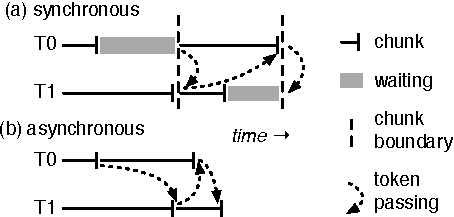
\includegraphics[width=3.0in]{figures/sync-async-chunks.pdf}
\caption{Synchronous versus asynchronous commit.}
\label{f:sync-async}
\end{figure}

Initial deterministic execution systems divided program execution into chunks consisting of a fixed number of instructions (typically 10-100,000) \cite{devietti_dmp:_2009,bergan_coredet:_2010,derek_r._hower_calvin:_2011} or separated by synchronization operations \cite{liu_dthreads:_2011}. 
After a thread executes one chunk it waits for all the other threads to execute their chunks before proceeding. This \emph{synchronous} approach (\autoref{f:sync-async}a) can lead to excessive waiting as threads often execute instructions or synchronization operations at different rates. An alternative \emph{asynchronous} approach was proposed by Merrifield and Eriksson \cite{merrifield_conversion:_2013} that eliminates global barriers, instead allowing threads to commit independently (\autoref{f:sync-async}b). In both synchronous and asynchronous approaches a global token circulates among threads in a deterministic round-robin order to ensure that commits occur deterministically.

\begin{figure}
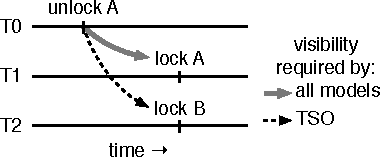
\includegraphics[width=3.0in]{figures/relaxed-consistency.pdf}
\caption{TSO requires that commits are global, while more relaxed models allow local commits that are visible to a subset of threads.}
\label{f:relaxed}
\end{figure}

Relaxing the consistency model improves the performance of determinism by making memory fences cheaper. Memory fence semantics define the number of threads to which commits must be made visible; with weaker consistency this number decreases which reduces the time it takes to push and pull commits. Consistency models like sequential consistency and total store order require that stores become visible in a total order that all threads agree on: commits must thus be a global operation (\autoref{f:relaxed}). Relaxed consistency models like DRF0 \cite{devietti_rcdc:_2011} and LRC \cite{kai_lu_efficient_2014} allow commits to be ``point-to-point'' with respect to a given synchronization object, i.e., the commit performed when releasing a lock need be visible only to the subsequent acquirer of that lock.

Removing global barriers and relaxing consistency offer orthogonal benefits and previous systems have explored these benefits both in isolation and in combination. \cite{merrifield_conversion:_2013} offers TSO with asynchronous commits, the RCDC system \cite{devietti_rcdc:_2011} adopts relaxed consistency but still uses synchronous commits, and RFDet \cite{kai_lu_efficient_2014} provides both asynchronous committing and relaxed consistency.

While RFDet could potentially provide the best performance of these schemes, the adoption of such an extremely relaxed\footnote{It is not obvious how further relaxations beyond LRC would be possible without breaking programming language semantics.} consistency model as LRC entails several additional costs. One concern is a space leak that arises from making commits visible only via a particular synchronization object. If a thread modifies some data and releases lock A, those modifications must be recorded until some other thread acquires lock A. This overhead is incurred for every lock release, causing space usage to scale with the number of lock objects. In the case that no other thread ever acquires lock A, space will be permanently leaked. This space overhead is not just a theoretical concern: in Section \ref{s:rfdet} we report large space overheads for RFDet on a benchmark with only a moderate number of synchronization operations.

 In addition to its space overheads, extremely weak consistency models like LRC are difficult for both humans \cite{adve_data_2010} and automated tools \cite{batty_mathematizing_2011,burckhardt_checkfence:_2007} to understand. The LRC model is substantially weaker than the most relaxed hardware consistency models (POWER and ARM) and thus programs compiled for a stronger model can break when executed on LRC. Recompilation with an LRC-aware compiler is necessary to generate the appropriate memory ordering instructions.

We propose that deterministic systems adopt stronger memory consistency models, such as the TSO model used in this work, to avoid these pitfalls. Next, we give an overview of the \lib system before discussing the optimizations that allow \lib to rival the performance of relaxed consistency approaches.

% We show that deterministic implementations of TSO can outperform weaker models because the cost of pushing and pulling commits can be quite low without resorting to weak consistency \ref{todo}. Furthermore, \textbf{the main performance bottleneck is the cost of deterministic synchronization} which requires centralized coordination in strong and weak consistency models alike. We show in \ref{todo} how to reduce the logical-physical clock skew that makes deterministic synchronization expensive. \TODO{may want to expand on clock skew here}

%%% Local Variables: 
%%% mode: latex
%%% TeX-master: "paper.tex"
%%% End:


\section{Speculative Determinism}

We can leverage the fact that strong DMT systems already provide isolation between 

%\newsavebox{\beginSpeculation}
%\begin{lrbox}{\beginSpeculation}% Store second listing
%\begin{lstlisting}
%void beginSpeculation(){
%}
%\end{lstlisting}
%\end{lrbox}
%
%\newsavebox{\commitSpeculation}
%\begin{lrbox}{\commitSpeculation}% Store second listing
%\begin{lstlisting}
%void commitSpeculation(){
%}
%\end{lstlisting}
%\end{lrbox}
%
%\begin{figure}
%\hspace*{.5cm}
%\usebox{\beginSpeculation}
%\caption{beginSpeculation() implementation.}
%\label{f:beginSpeculation}
%\end{figure}
%
%\begin{figure}
%\hspace*{.5cm}
%\usebox{\commitSpeculation}
%\caption{commitSpeculation() implementation.}
%\label{f:commitSpeculation}
%\end{figure}

%first paragraph, outline the goals....what are we trying to achieve

%next, how does speculation work?

\subsection{Memory Model}

\subsection{Adaptation}

\section{Implementation}
\section{Evaluation}


%Outline some drawbacks, mainly performance and what folks have done to fix things


%\acks

%Acknowledgments, if needed.

% We recommend abbrvnat bibliography style.

\bibliographystyle{abbrvnat}

% The bibliography should be embedded for final submission.



\end{document}
